\subsection{Overview}
\begin{figure}[H]
    \centering
    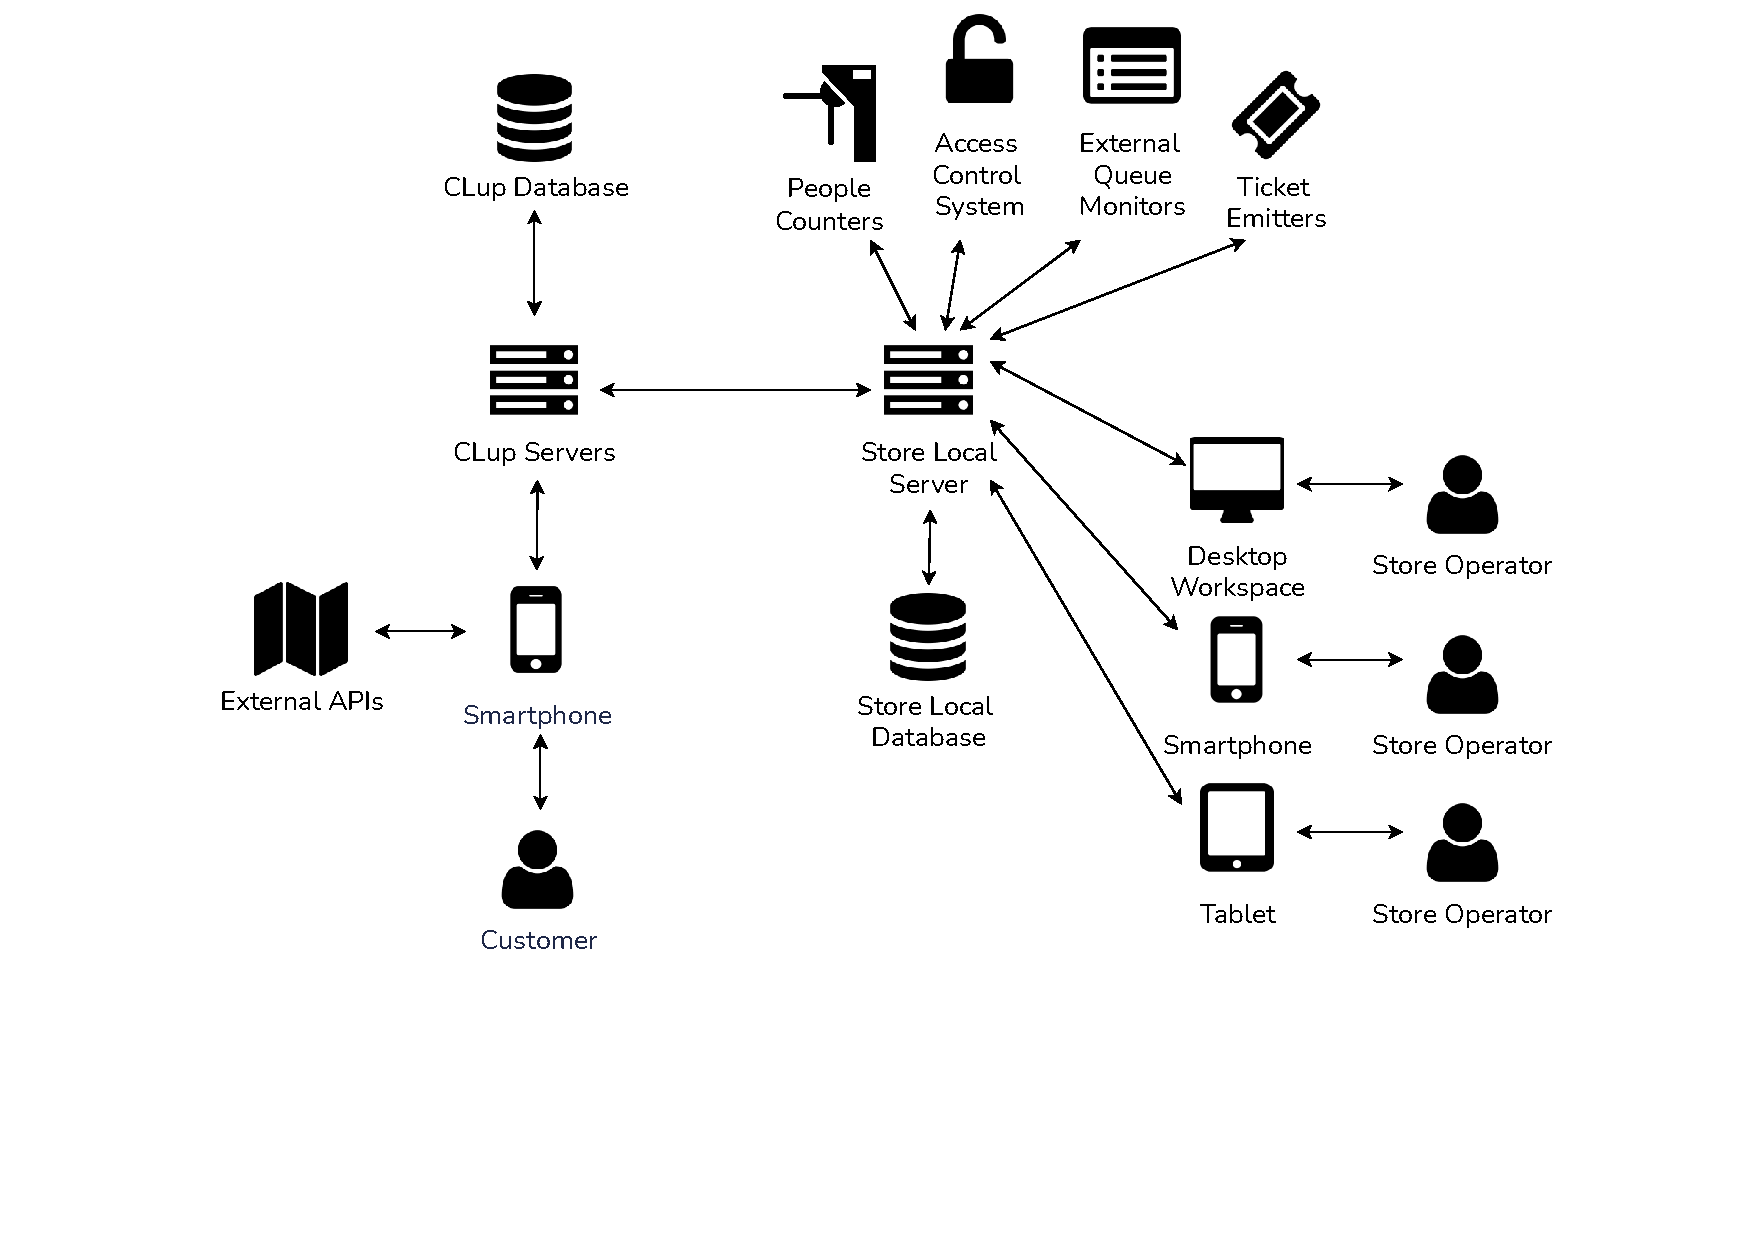
\includegraphics[scale=0.6]{Images/overview.pdf}
    \caption{\label{fig:Overview} CLup System Overview}
\end{figure}

This diagram shows the CLup system as a whole, its actors and main components, from an high level perspective. 

Store customers interact with the system by using a smartphone, which depends on external third party APIs to visualize and interact with maps.
Store operators can interact with the system using different kinds of devices, to better suit their needs when working at the shop: smartphones can be handy when they need to check information about the store queue while moving through departments; tablets make looking at graphs and statistics more easily without loosing the 'mobile' factor, and having a CLup application also on desktops can also be convenient for operators working at a desk (without having to switch from one device or another in their workflow).

CLup Customer Application communicates directly with CLup servers through REST APIs, while CLup Operator Application connects to the Store Local Server which retrieves data both from the Store Local Database and from CLup Servers. 

Store Devices also connect to the Store Local Server, to enhance the functionalities and automate tasks such as admitting customer entrances, monitoring the people inside the store departments, handing out tickets.

CLup Servers on the other hand only store data that is needed to permit queue regulations, for example information about occupancy limits, live occupancy of the stores, markets locations.

Following sections will analyze every major component more deeply, describing in detail its underlying sub-components and interfaces.  

\subsection{Component View}
\begin{figure}[H]
    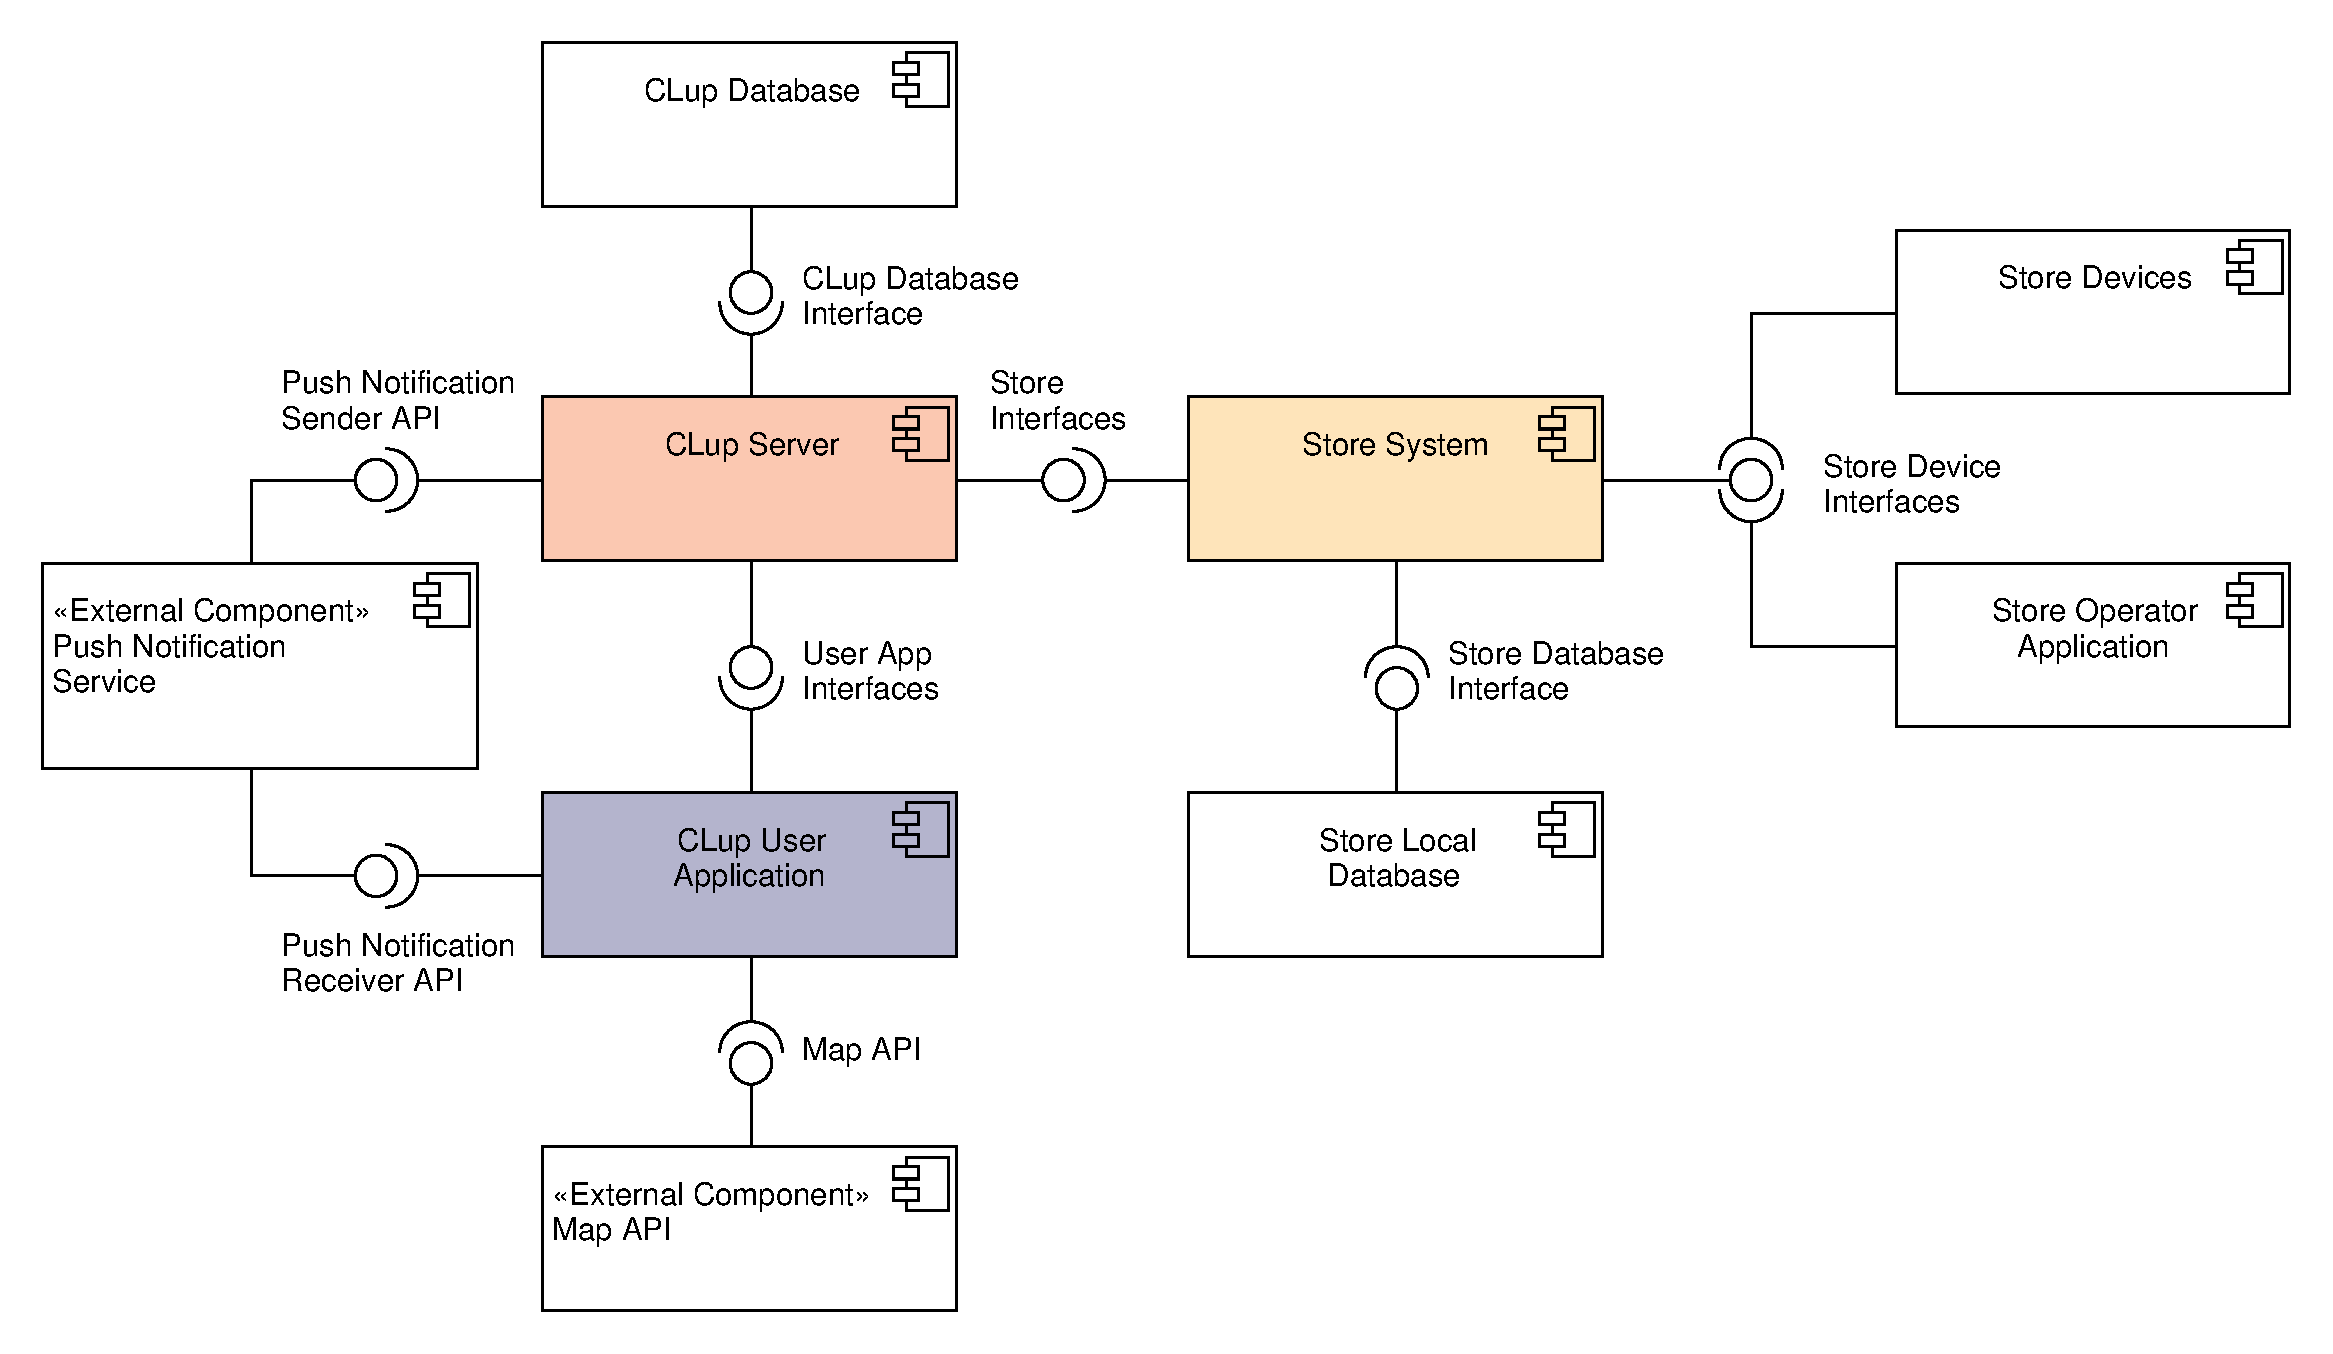
\includegraphics[width=\textwidth]{Images/UML_general_component.pdf}
    \caption{\label{fig:UML_comp_general}General component diagram}
\end{figure}
Figure~\ref{fig:UML_comp_general} shows a general, simplified, component view of the S2B.
The three main components of the system are: the CLup User Application, the CLup Server and the Store System with their databases. CLup system also interacts with external components like Map API Services and other physical components (i.e.~store devices).

Customers use the \textbf{CLup User application} to check supermarkets near them and eventually book a visit or retrieve a ticket. The User application interfaces with the \textbf{CLup server}. 

Sometimes the customer need to receive notifications about their ticket, to allow this the CLup Server and the application need to use the Push Notification service, each OS manifacturer provide his different push notification service. This service provides its dedicated API for sending and receiving push notifications.

The CLup server is the central component of the system, mediating between the customers and the stores. It manages customer authentication, tickets issued remotely by the CLup application, and hands out to the public information about stores to the customers (i.e.~opening hours, waiting times, etc). 

The \textbf{Store system} provides an interface for all the physical devices in the store, collecting and processing data from them and then routing the data to the CLup server or keeping it in the local database. The system communicates with a local database to store temporary data about tickets, the statistics collected and the authentication details of the store operators.

\subsubsection{CLup Server component view}
\begin{figure}[H]
    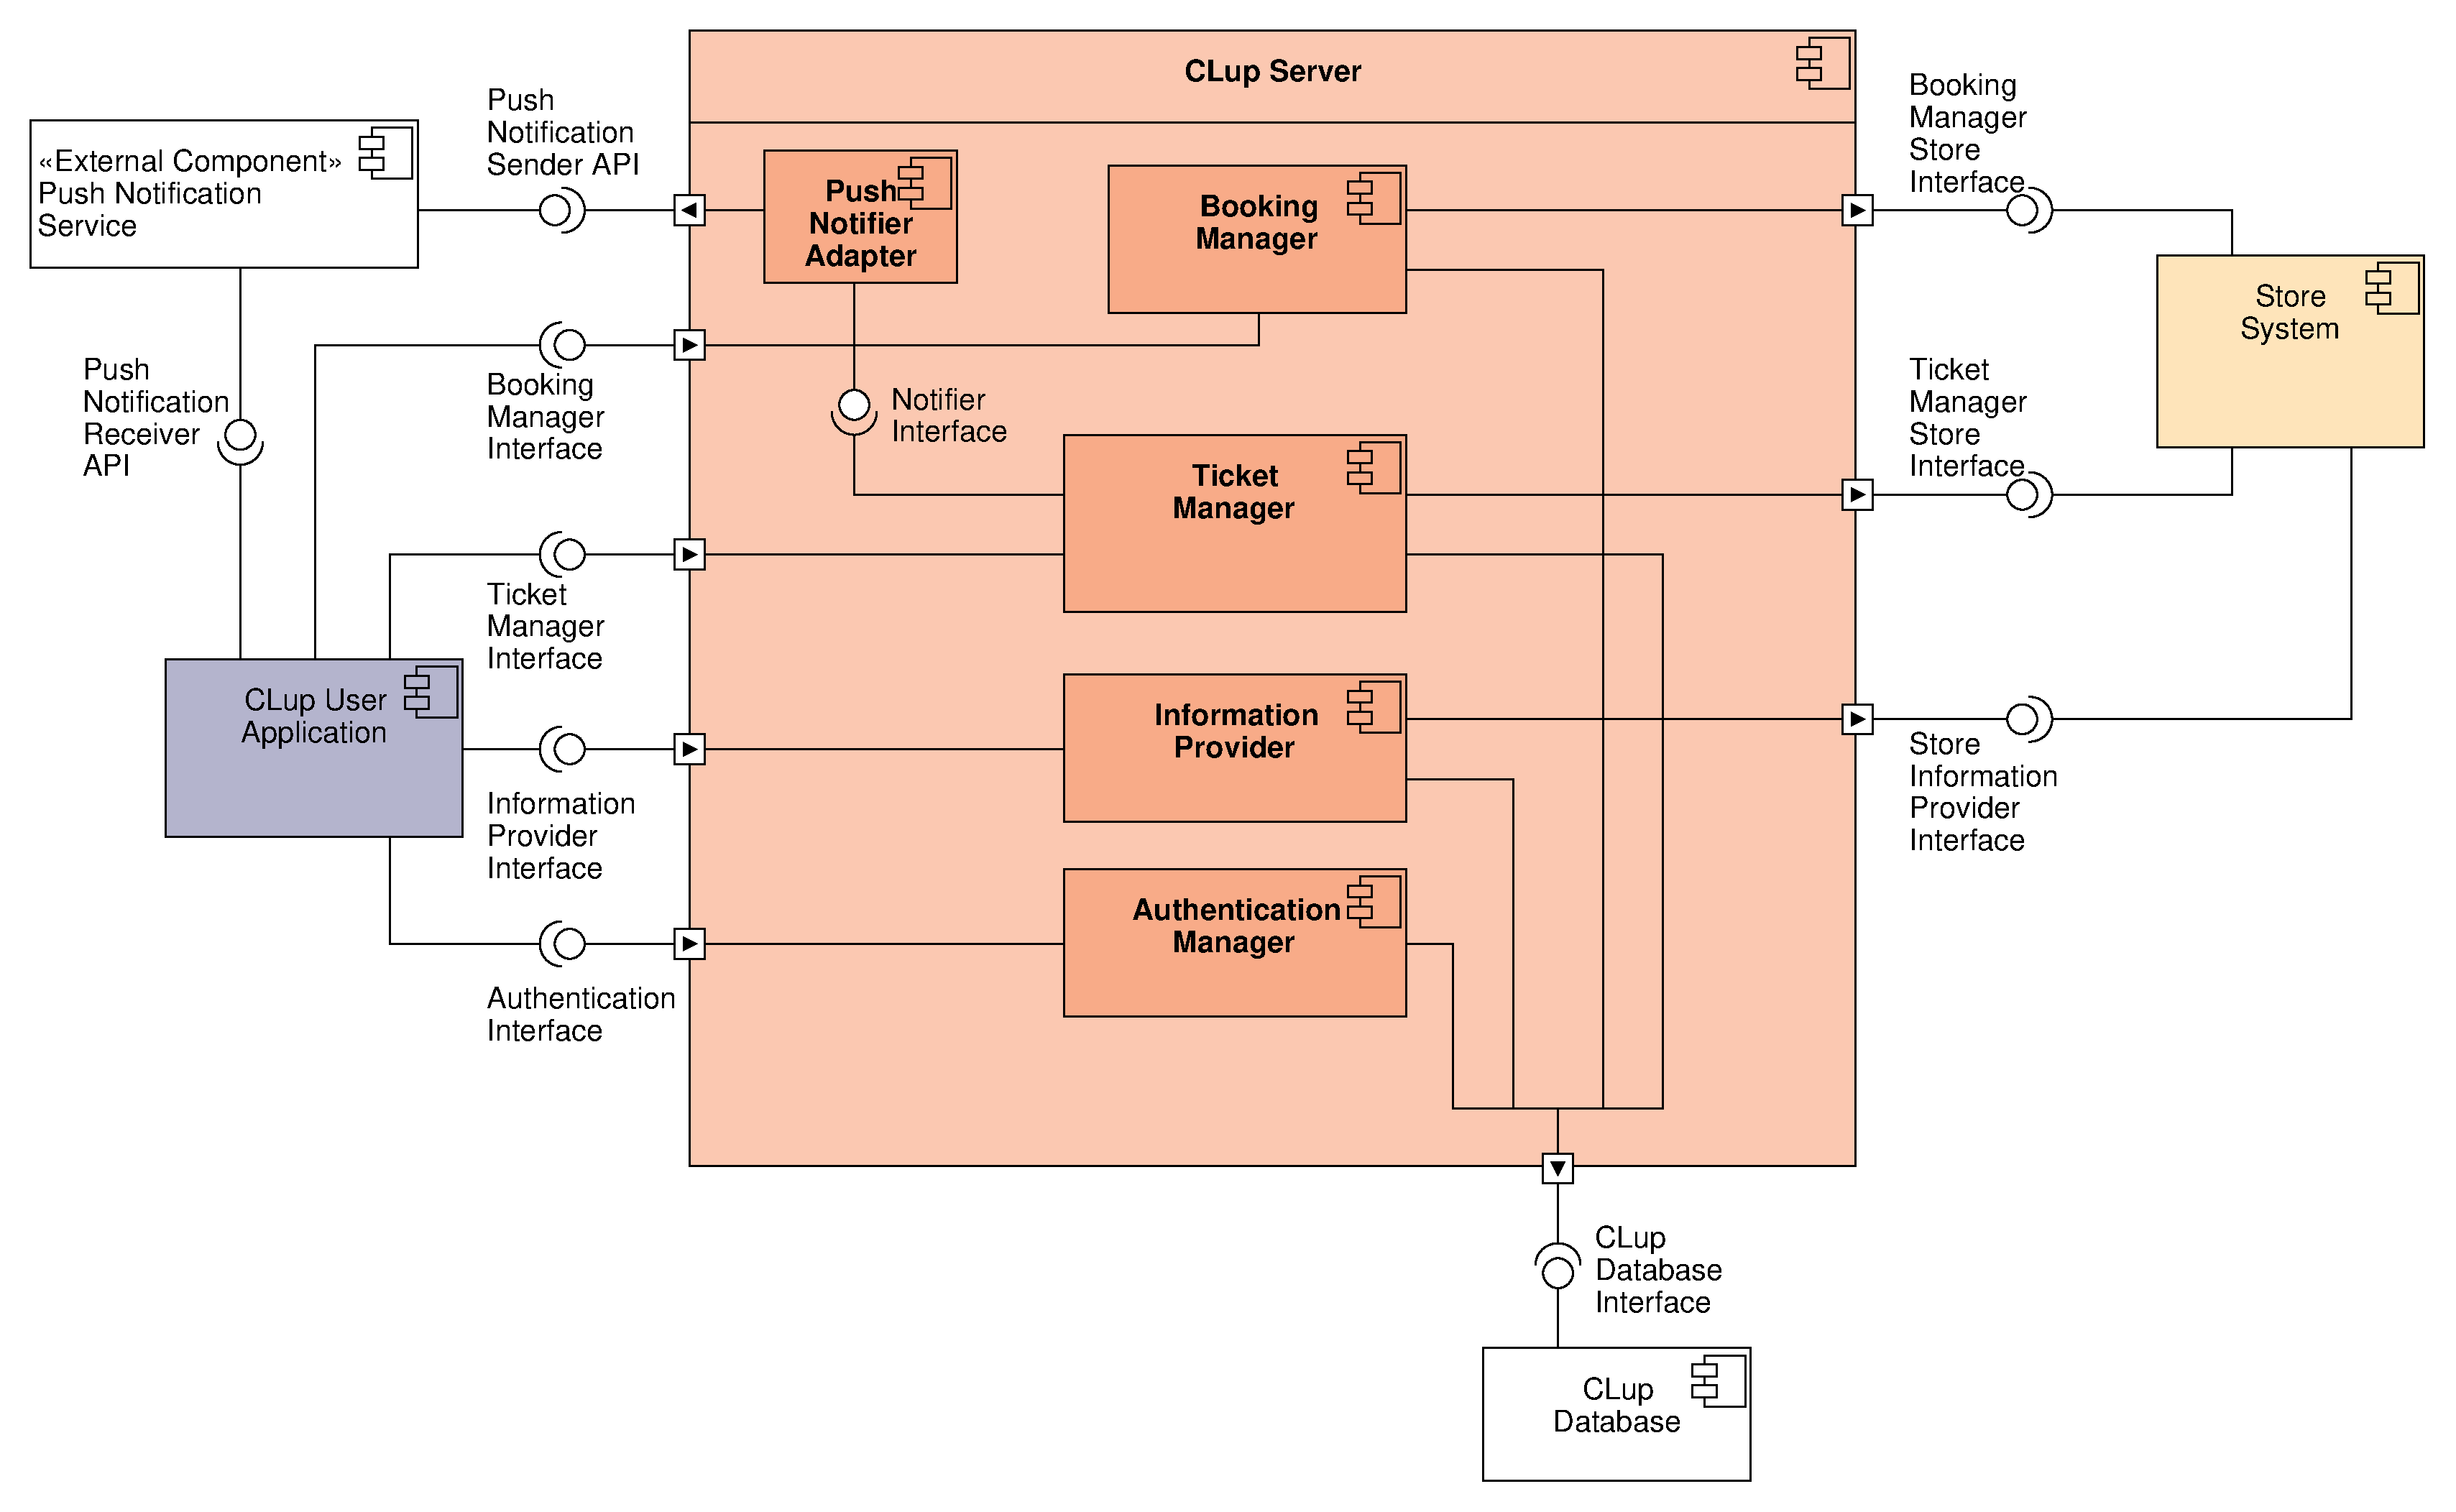
\includegraphics[width=\textwidth]{Images/UML_server_component.pdf}
    \caption{\label{fig:UML_comp_Clup_server}Component diagram for CLup server}
\end{figure}

The CLup server provides interfaces to the CLup User application and to each Store System. This component stores the persistent data in the CLup Database component communicating with it using a common Database interface.

The CLup Server has these internal components:
\begin{itemize}
    \item \textbf{Authentication Manager}: handles customer registration and authentication. To do this task this component needs to communicate tightly with the CLup database which stores the user data and their hashed passwords;
    \item \textbf{Information Provider}: hands out information to the customers requesting them. These information can be of various nature, like opening hours or the store crowdedness in various times of the day. This data is retrieved from the CLup database or from the Store System which uses another interface to push them periodically.
    \item \textbf{Ticket Manager}: issues virtual tickets when customers requests them. This component interfaces directly with the Store System, adding the created tickets to the queue. The component has the responsibility to notify the customers when it's time to approach the store entrance; it uses the notification interface, provided by the Notifier component.
    \item \textbf{Booking Manager}: handles the visit booking. Queries the database about free slots in the day when a customer wants to make a reservation. Requests are eventually finalized by attaching the shop list to the booking if and when the customer adds it from the application. This components also pushes updates to the Store System about changes regarding the bookings (e.g. cancellation, shopping list changes, etc).
    \item \textbf{Notifier}: handles all the aspects about sending push notifications to the users, taking into account that the CLup application can be running on different operating systems and that they provide different services to receive these notifications. The notifier needs to communicate with the external Push Notification Service, using the interface provided by that service.
\end{itemize}

\subsubsection{CLup customer application component view}
\begin{figure}[H]
    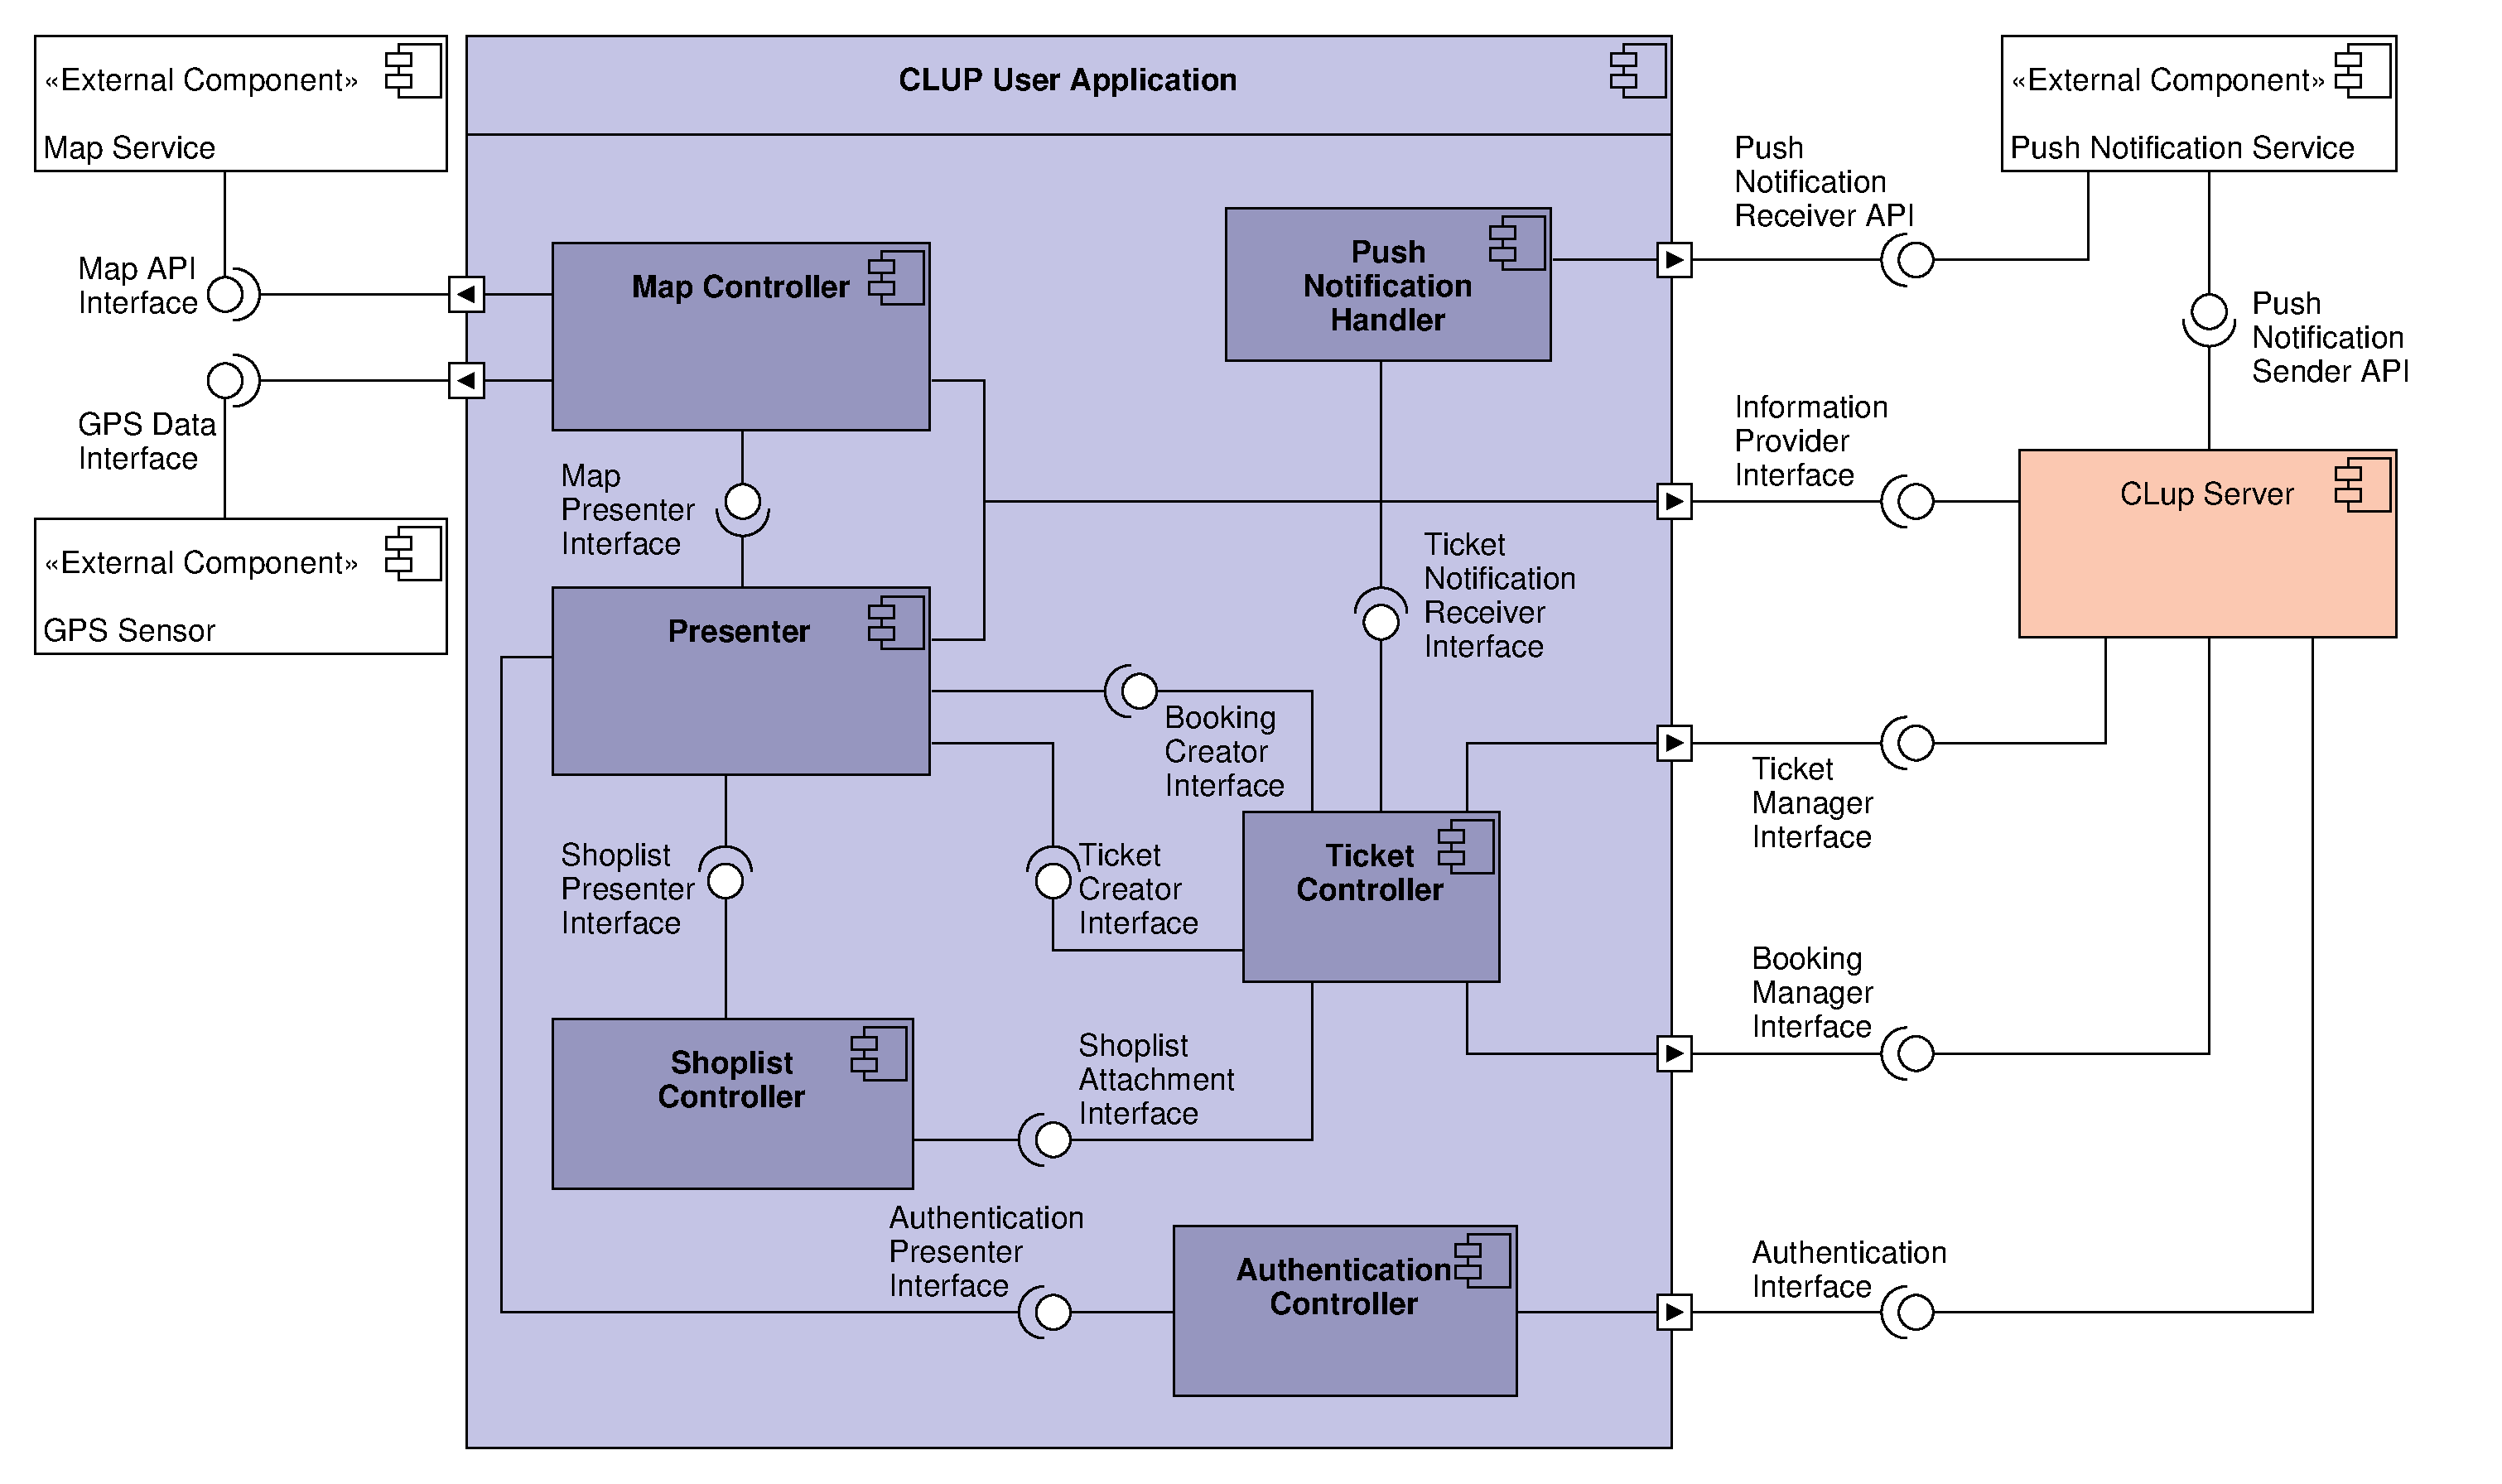
\includegraphics[width=\textwidth]{Images/UML_user_app_component.pdf}
    \caption{\label{fig:UML_comp_CLup_user_app}Component diagram for CLup User Application}
\end{figure}

The CLup user application provides the functionalities of CLup to store's customers. The applications needs to interface with the GPS Sensors and to an external map service that provides a map containing all the stores. The application also needs some controllers that will communicate with the CLup server to retrieve store information, authenticate, book a visit or create a queue ticket.

The user application contains these sub-components:
\begin{itemize}
    \item \textbf{Authentication}: allows the user to create a CLup account and to log-in with an existing account.
    \item \textbf{Map Controller}: Handles the communication with the external Map Service and the GPS. Exploits the Map API provided from the Map Service to get the map data near the user position then will request data to the CLup server in order to populate the map with the nearby stores.  access data about the location of the user. For this task the component will use the Information Provider Interface offered by the CLup server component.
    \item \textbf{Presenter}: Handles the GUI of the applications and the events from the user like the push of a button or the text boxes. Needs to relate with all the controllers components that handle different the different aspects and functionality of the application. To do this these component will provide their interface exposing all the functionalities that each controller offers.
    \item \textbf{Shop-list Controller}: manages the creation of shop lists that will be attached to visit bookings in order to estimate the occupancy of the various department of the store.
    \item \textbf{Push Notifications Handler}: handles and displays to the user the push notification received from the CLup Server about the bookings or the tickets created from the user. This component is provided by the underlying Operating System, and the interface is accessible through standard libraries of the application programming language.
\end{itemize}

\subsubsection{Store System component view}
\begin{figure}[H]
    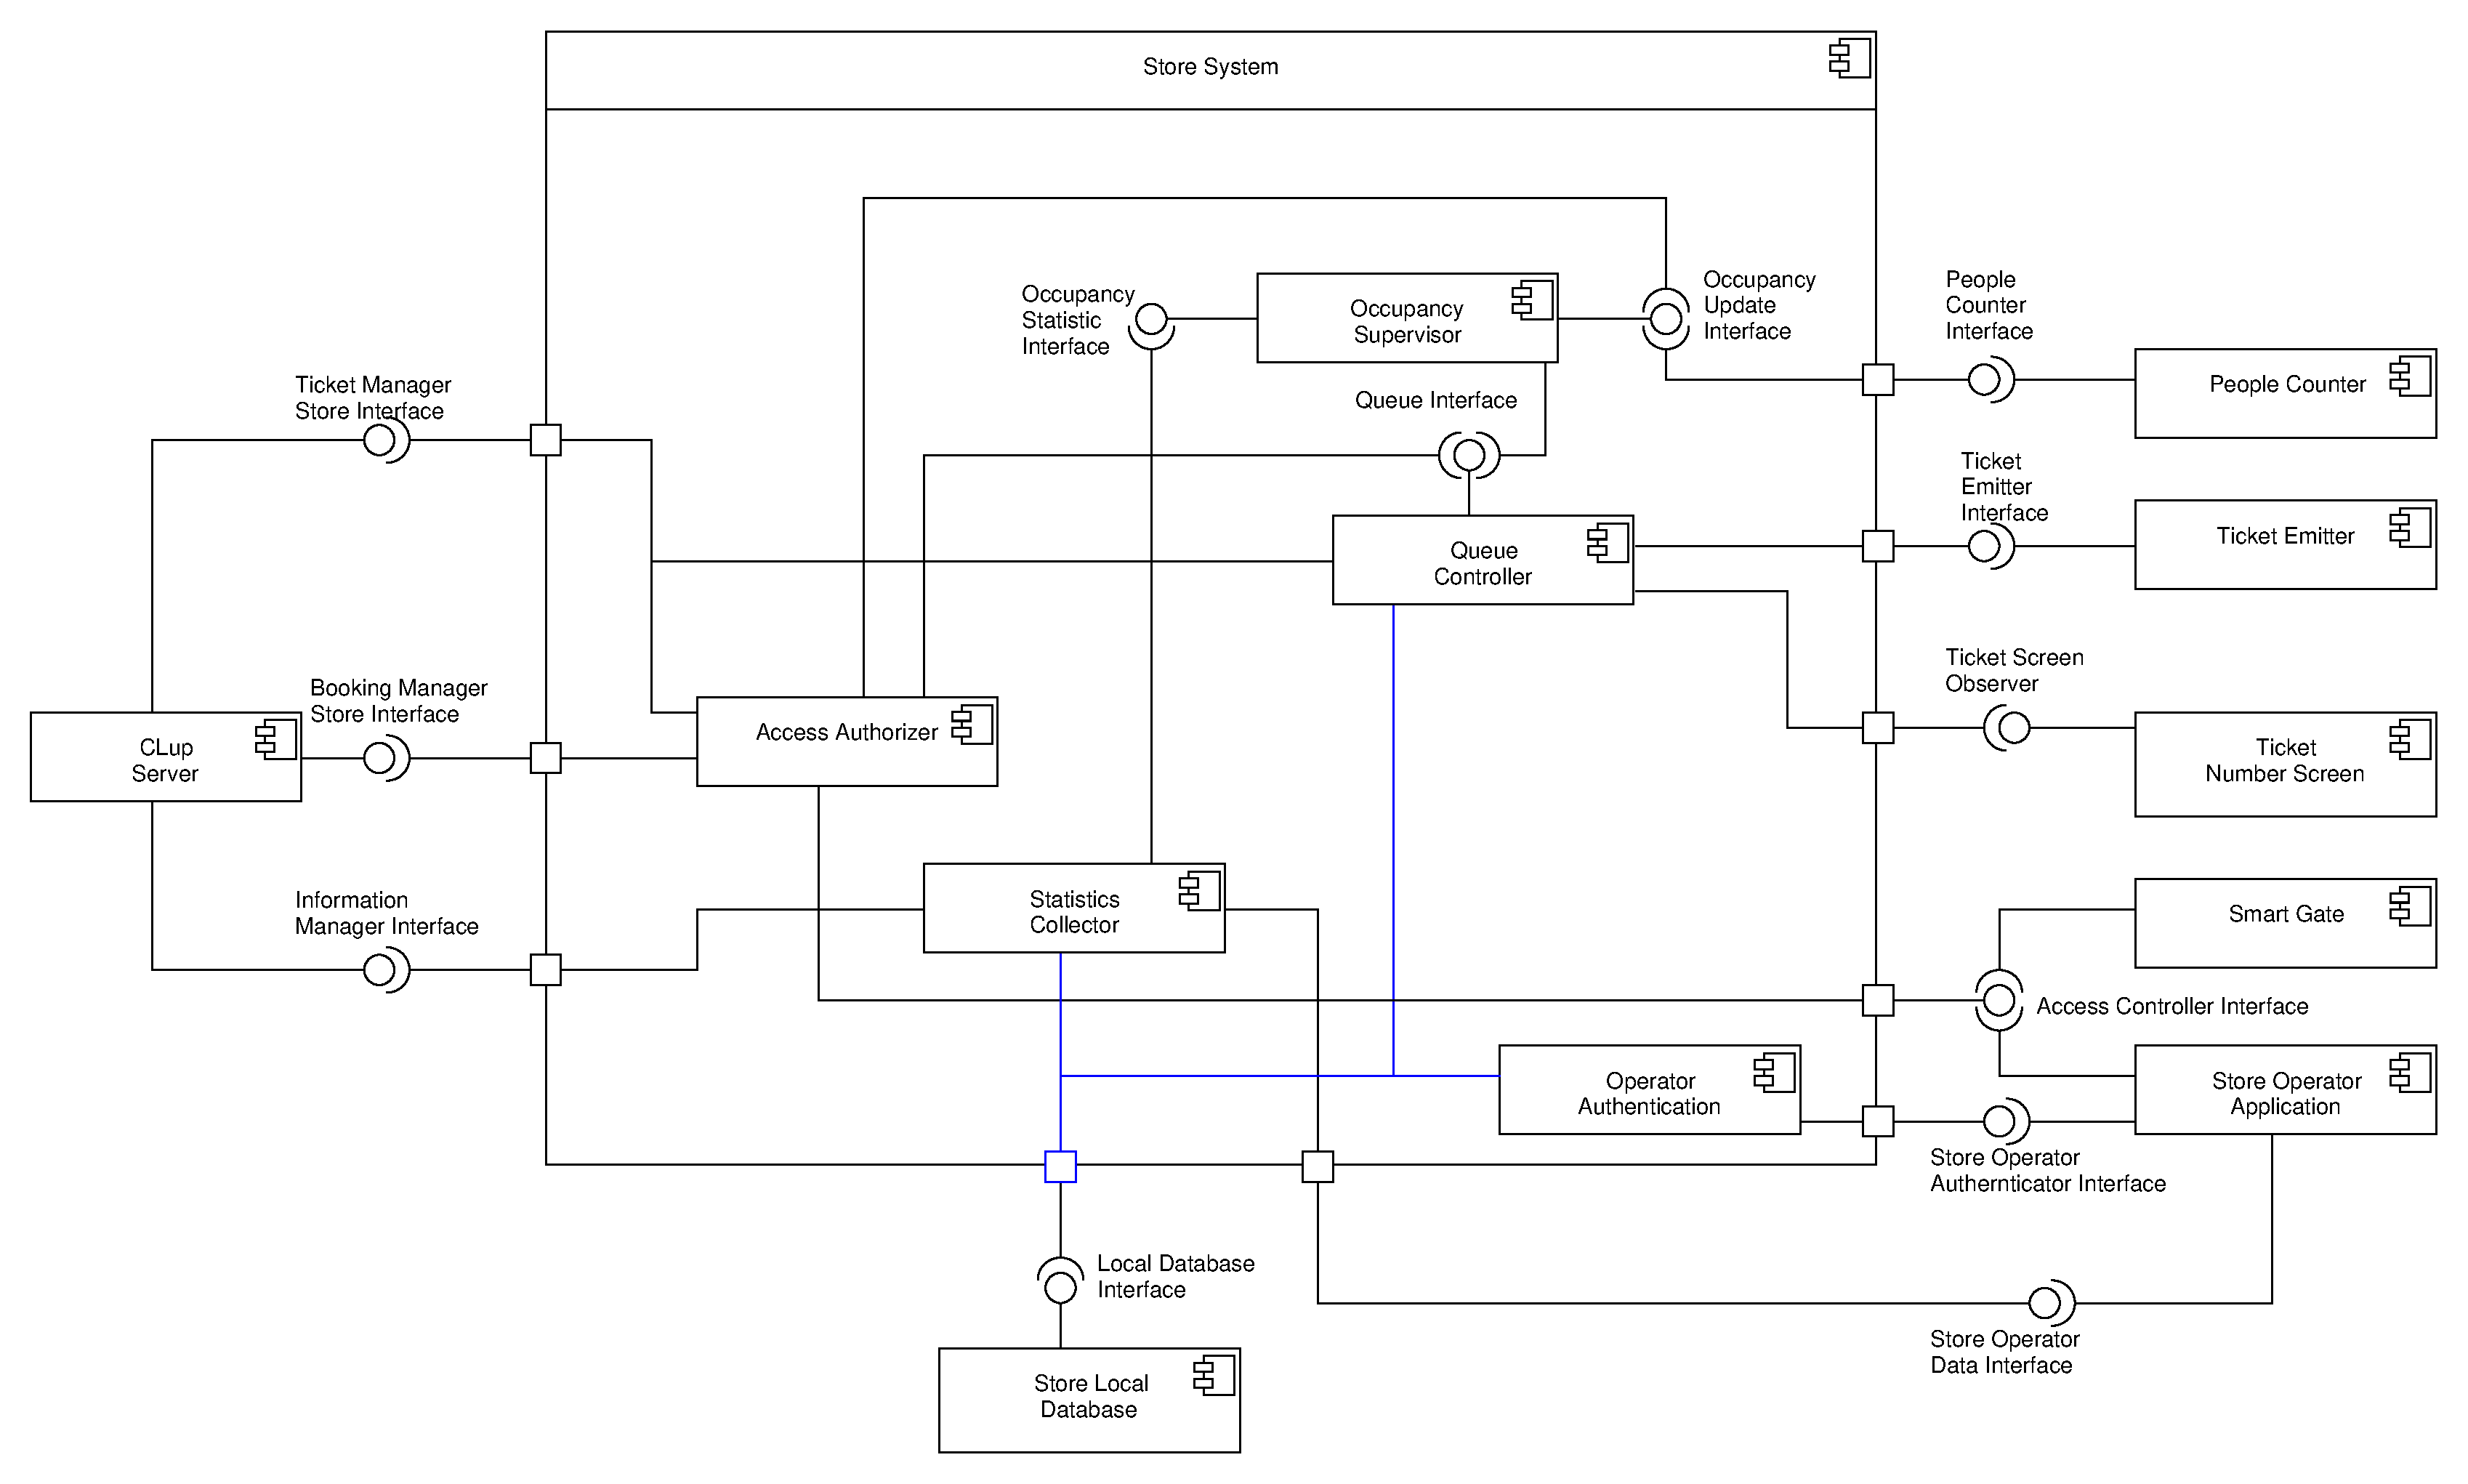
\includegraphics[width=\textwidth]{Images/UML_store_system_component.pdf}
    \caption{\label{fig:UML_comp_CLup_store_system}Component diagram for Store system}
\end{figure}

The Store System receives data from the store physical devices and combines it with the information retrieved by the CLup Servers. This component uses the interfaces provided by the CLup Server and lays out its own interfaces that are used by the physical devices located in the store. This component interfaces with a local database containing store statistics, store operators authentication data and local data that need persistency.

\begin{itemize}
    \item \textbf{Operator Authentication}: allows store operators to authenticate using their store credential. This component communicates with the Store Operator Application, which is used to manually check tickets and register the customer admissions in the store. The component fetches the authentication data in the store local database, using the interface provided by the database.
    \item \textbf{Occupancy Supervisor}: checks that the occupancy limits are not violated using all the data that it receives about people entering and leaving the store. This data can be provided directly by devices like People Counters, or from the Access Authorizer. The latters increments the counter of the number of people inside the store when an access is authorized. The Occupancy Supervisor checks information about the bookings and notifies the Queue Controller when there is space to admit new customers with a numbered ticket (without a booked visit).
    \item \textbf{Queue Controller}: handles the queueing of the customers by combining the data about virtual numbered tickets and paper numbered tickets, using the proper interfaces to communicate with the CLup Server. The Queue Controller is notified by the Occupancy Supervisor when customers in line can be called to the entrance; it then updates the ticket numbers on the screen placed at the store entrance (with the new numbers obtained using its interface).
    \item \textbf{Access Authorizer}: receives the code read by the Access Controller (that can be either a Smart Gate or a store operator), checks if that code is valid and allowed to enter, then notifies back the Access Controller. Even if the ticket is valid, before admitting a customer, this component needs to check that the occupancy limits of the store will not be violated by letting customer inside the store, consulting the Occupancy Supervisor. The Access Authorizer will check (requesting information from the CLup server) if the ticket refers to a pre-booked ticket; otherwise it will check if the ticket is on top of the queue using the Queue Controller interface.
    \item \textbf{Statistics Collector}: collects and periodically elaborates statistics with data from the Occupancy Supervisor and Queue Controller. Statistics are saved in the store local database. Brief elaborated data that can be shown to the customer (i.e.~indications of the crowdedness of the store, estimated waiting times,\ldots) are sent periodically to the CLup Server using the Store Information Provider interface.
\end{itemize}
\subsection{Deployment View}

\subsection{Runtime View}
\begin{figure}[H]
    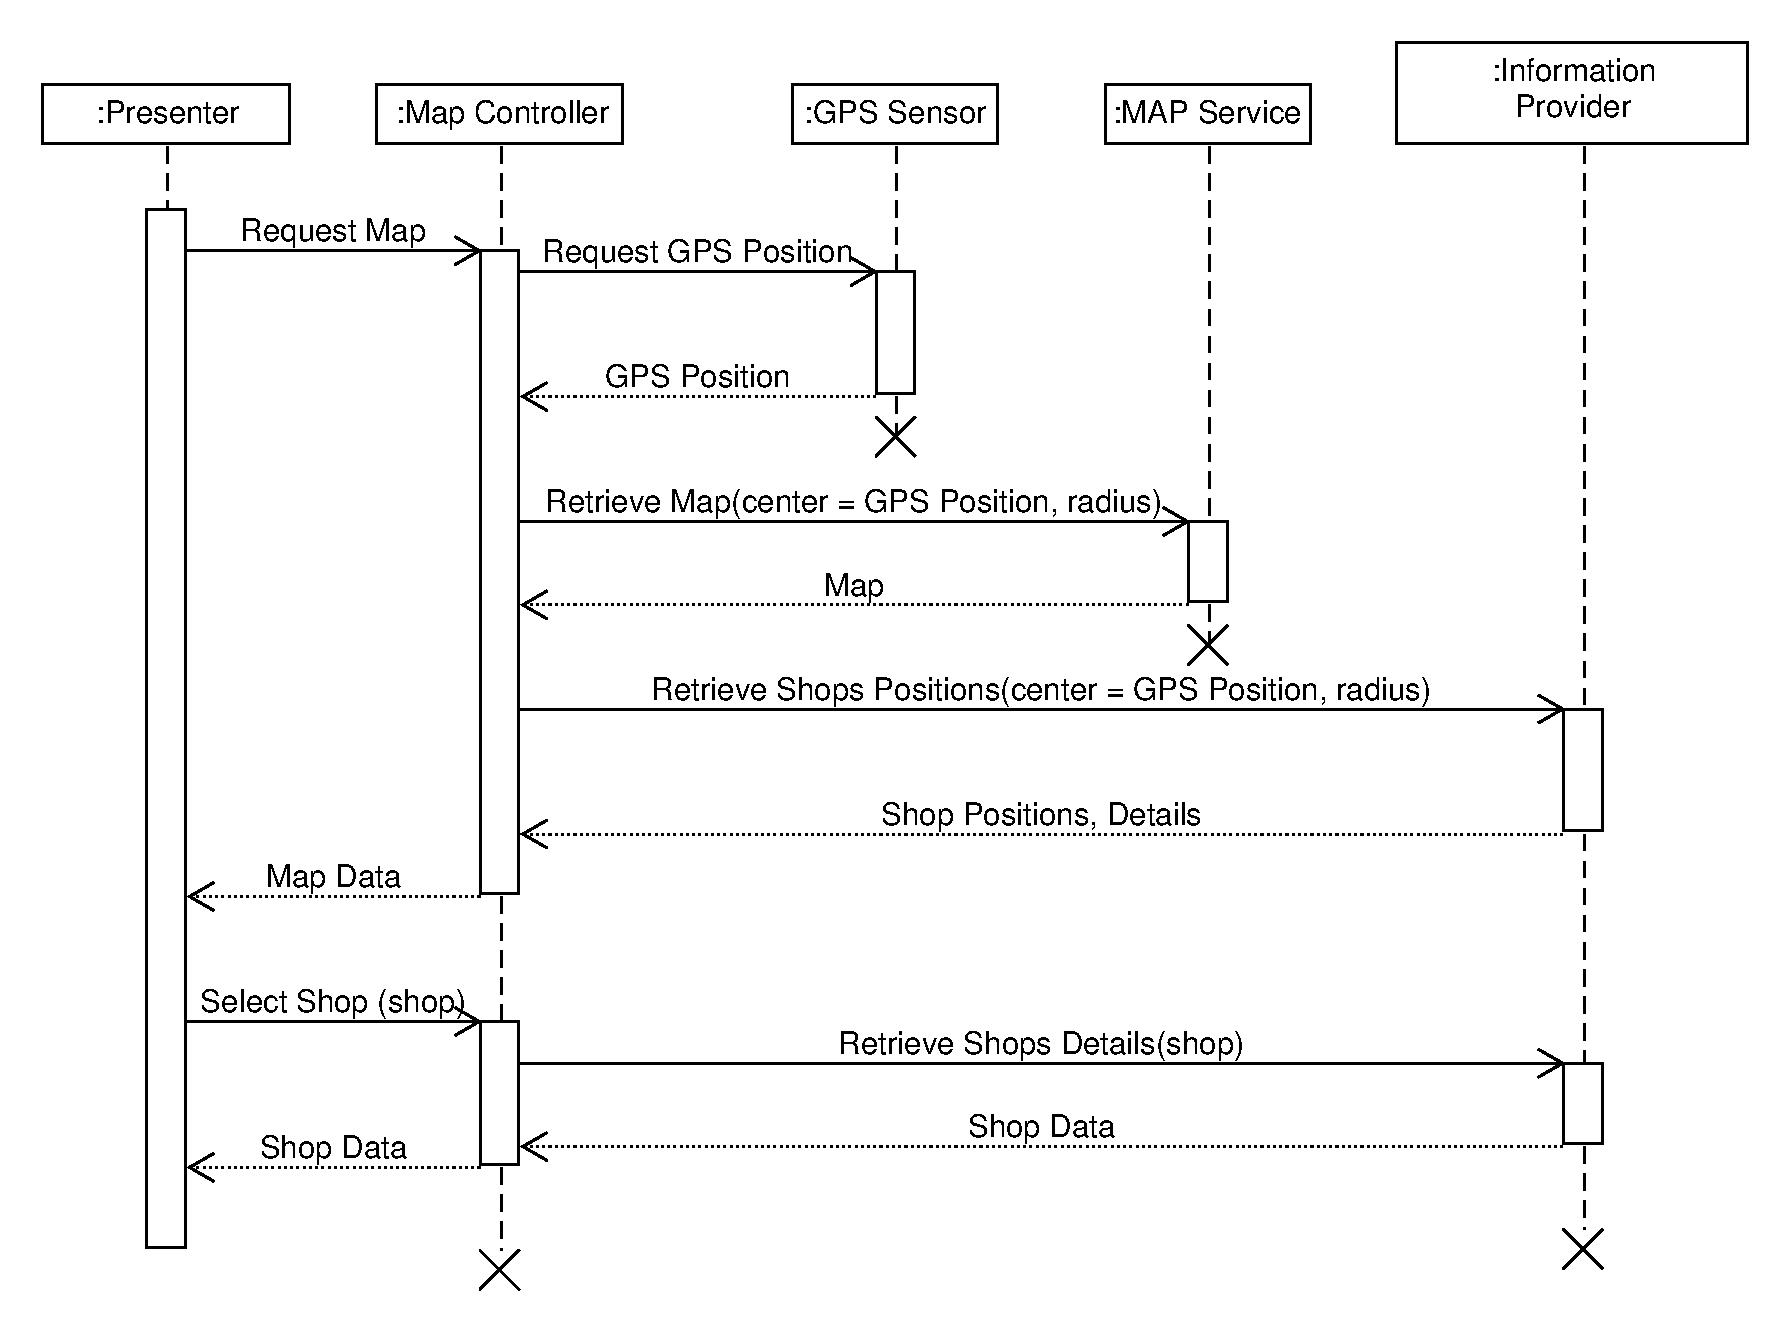
\includegraphics[width=\textwidth]{Images/UML_user_map_sequence.pdf}
    \caption{\label{fig:UML_user_map_sequence}Sequence diagram for store map loading}
\end{figure}
\begin{figure}[H]
    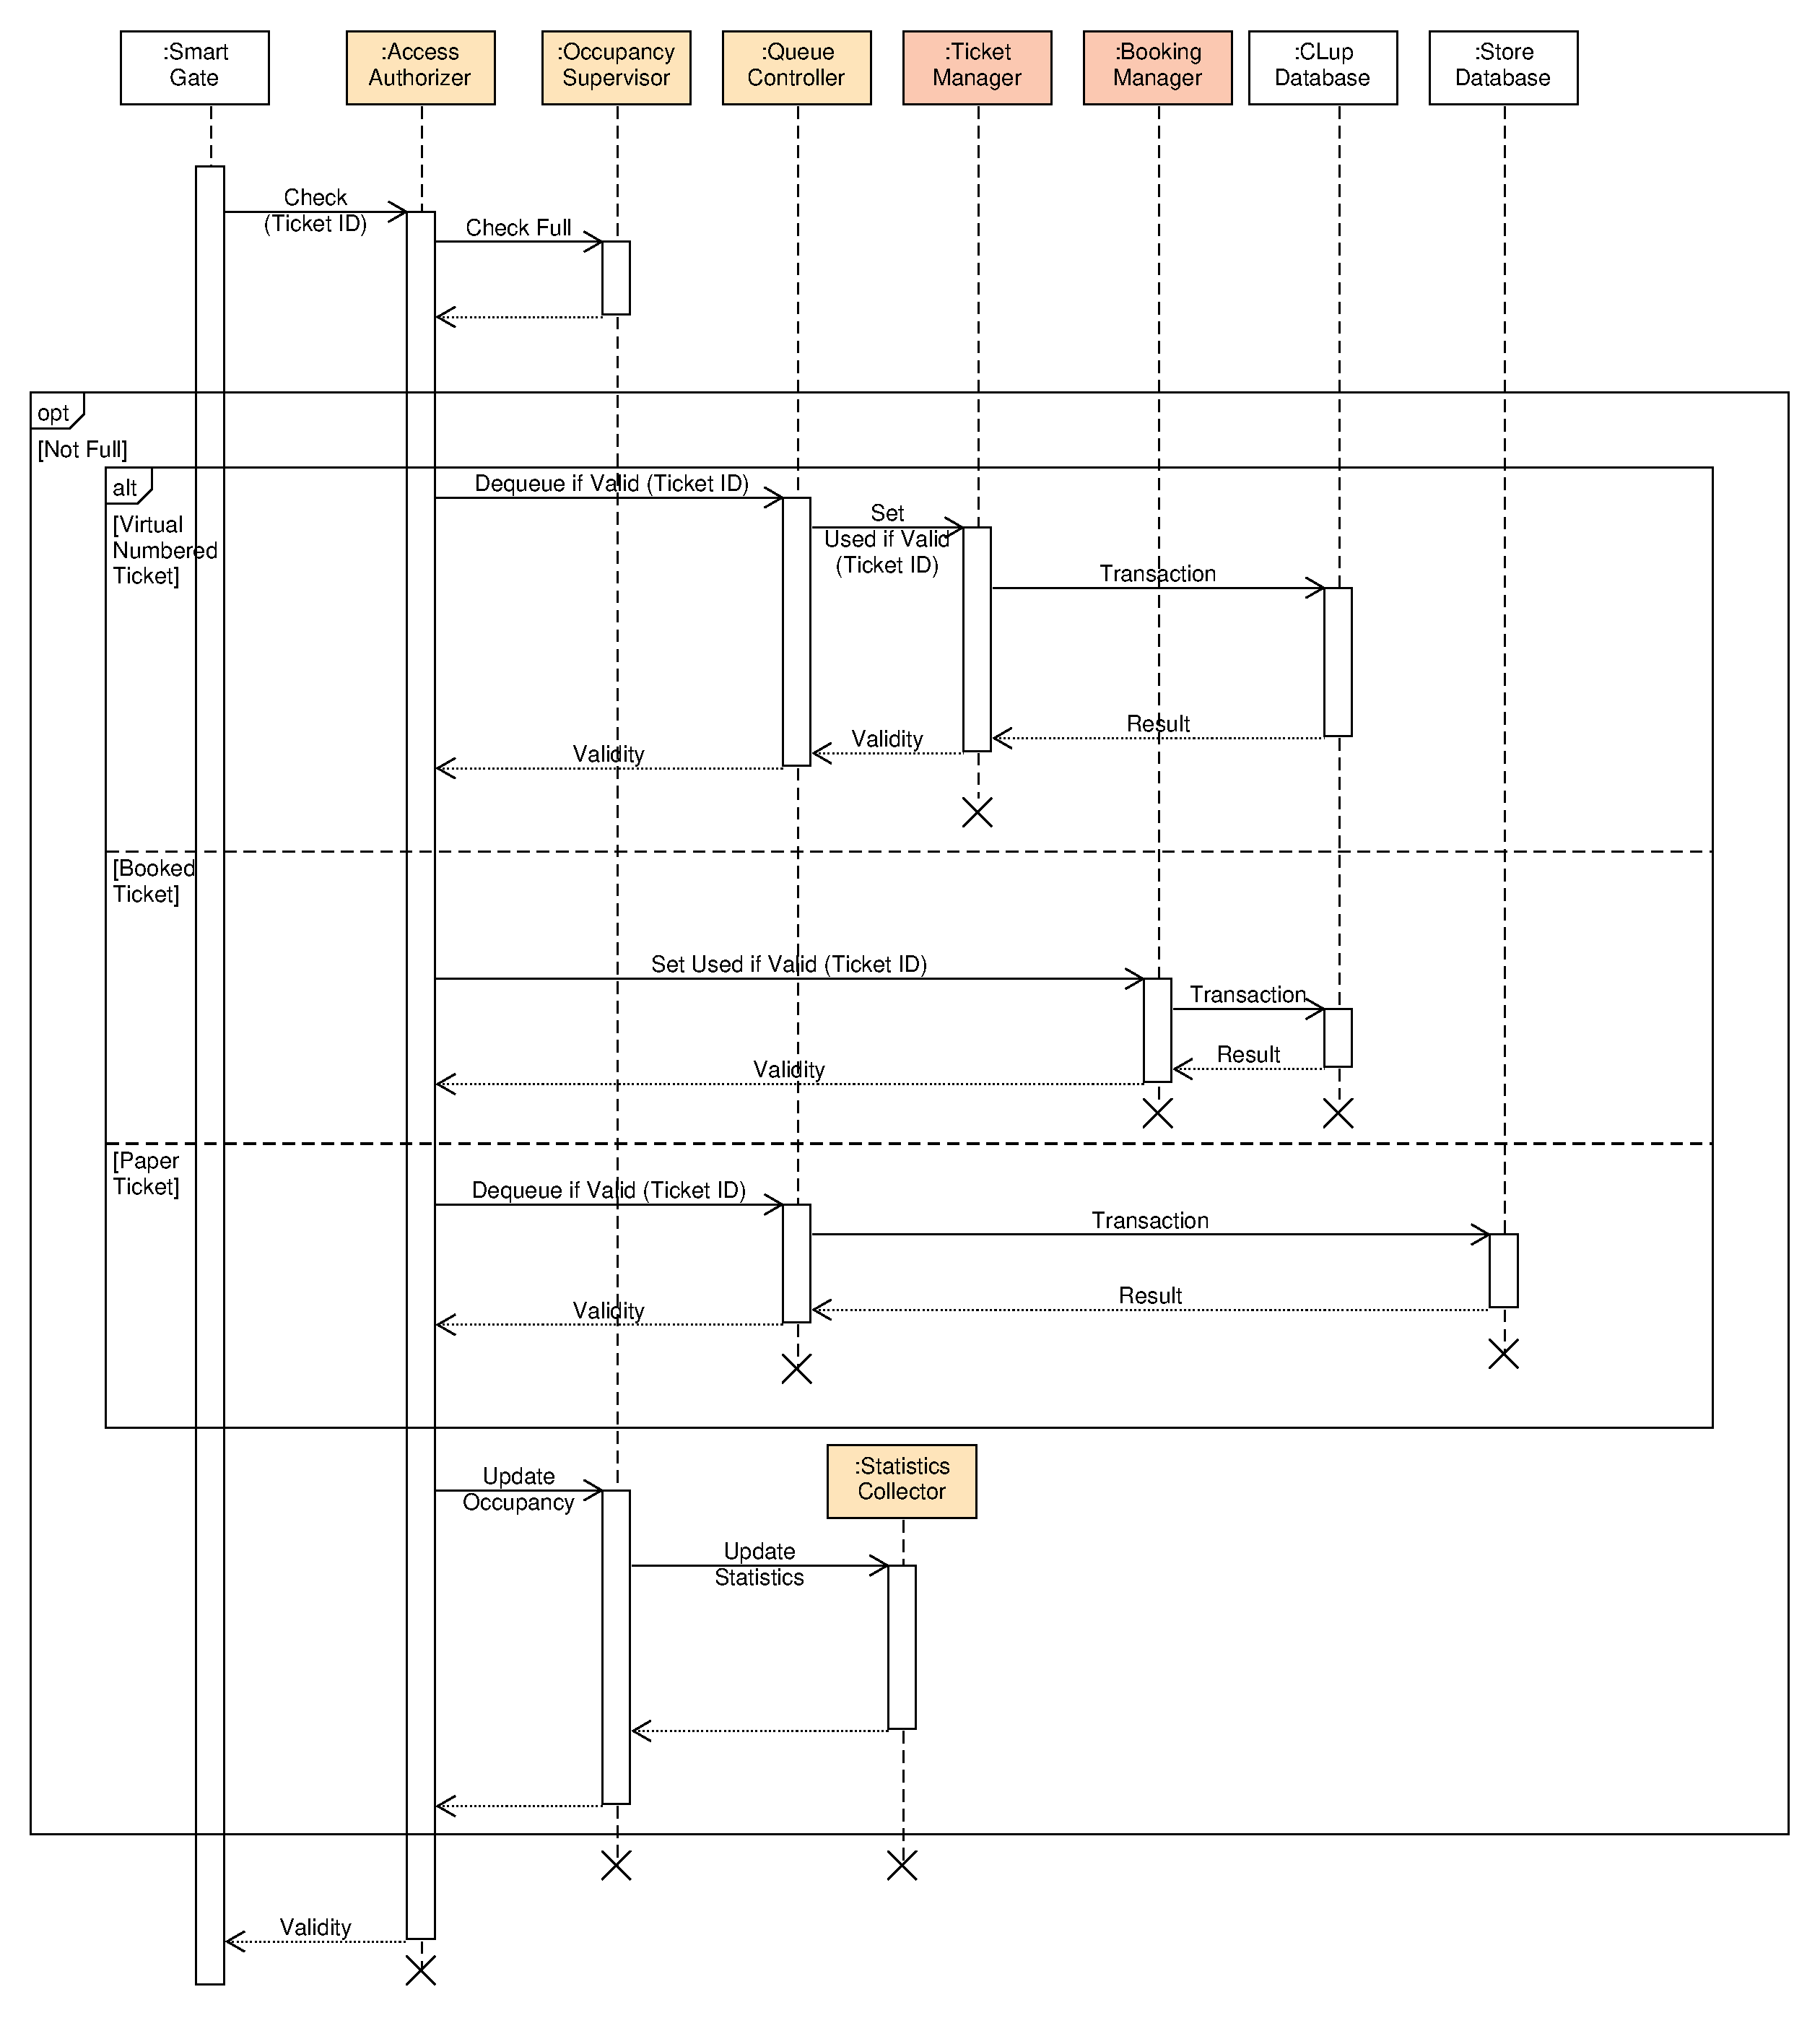
\includegraphics[width=\textwidth]{Images/UML_ticket_scan_sequence.pdf}
    \caption{\label{fig:UML_ticket_scan_sequence}Sequence diagram for store map loading}
\end{figure}
\begin{figure}[H]
    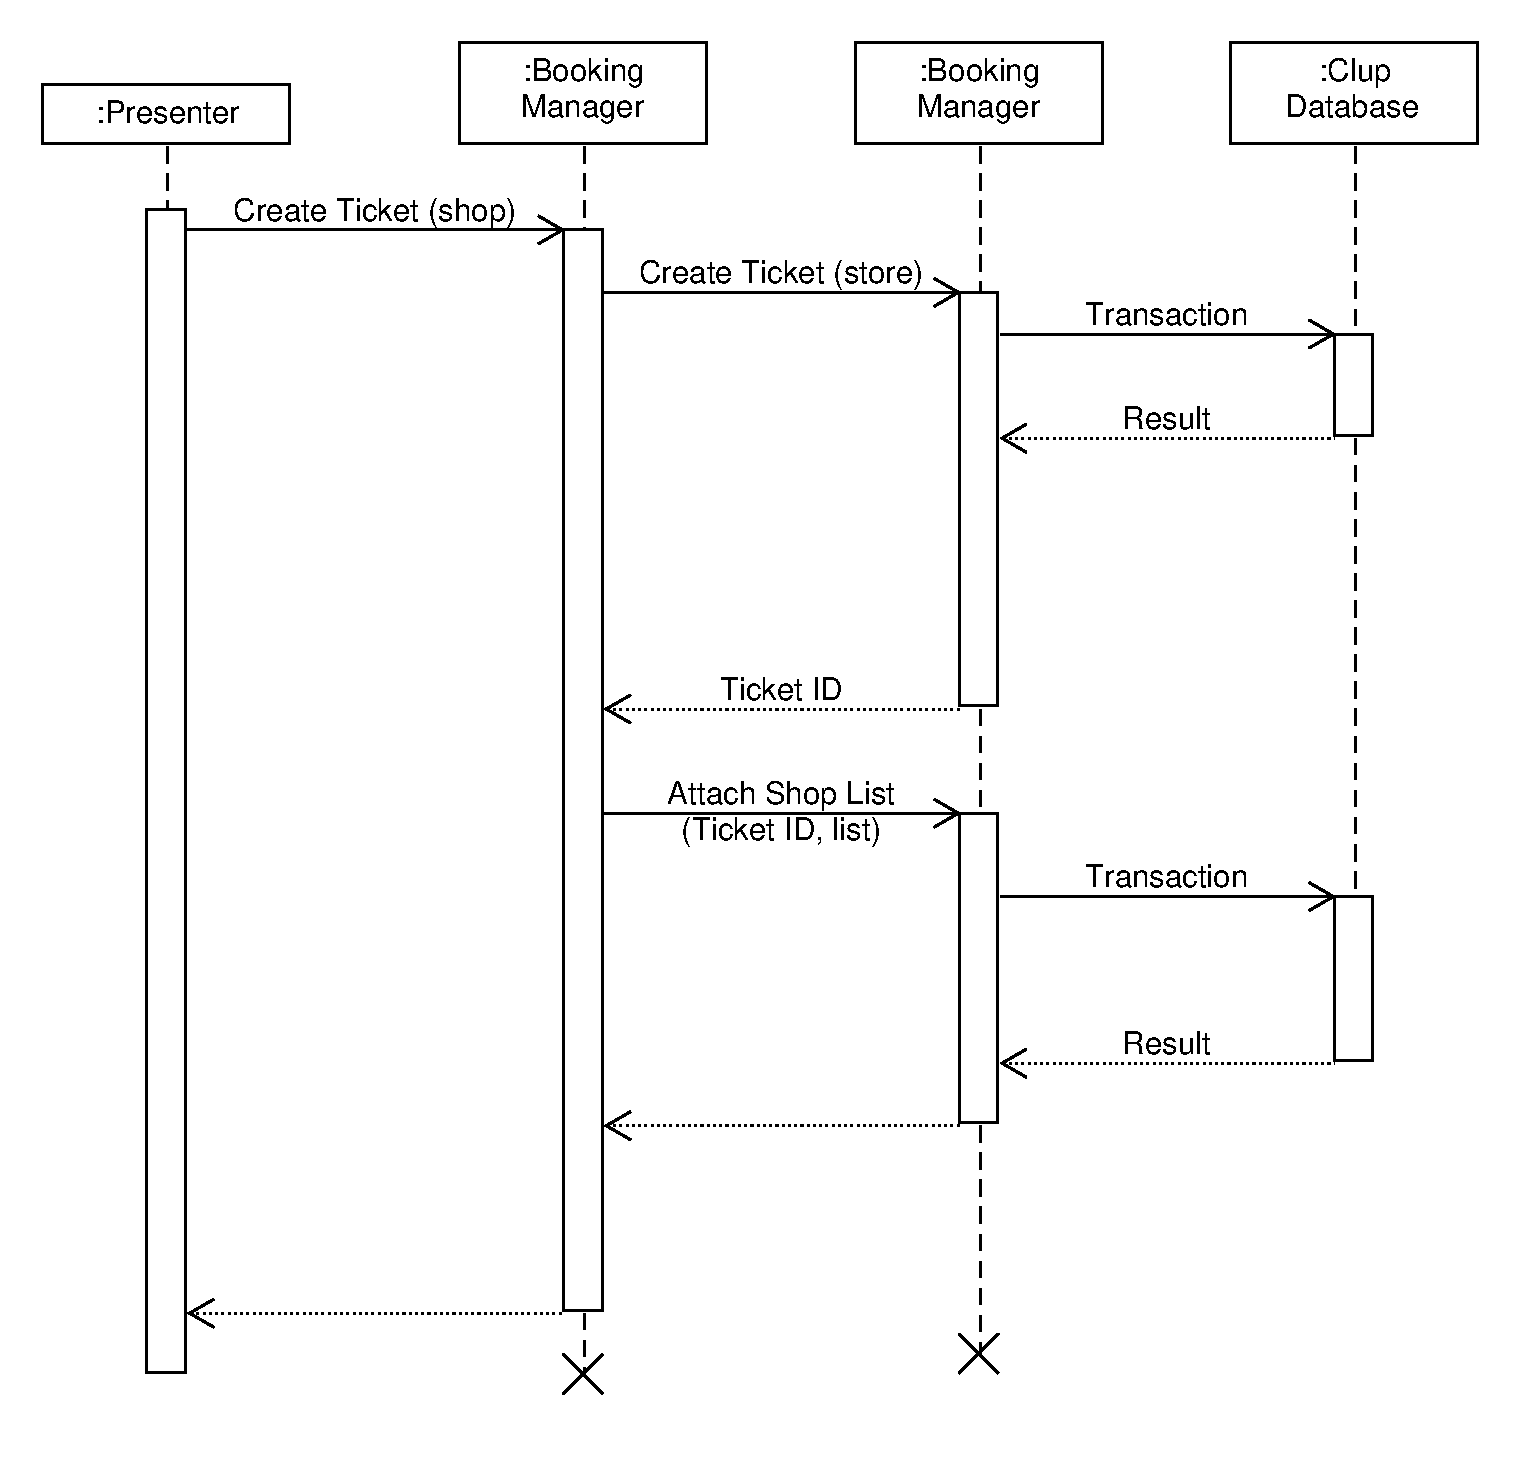
\includegraphics[width=\textwidth]{Images/UML_user_book_visit.pdf}
    \caption{\label{fig:UML_user_book_visit}Sequence diagram for store map loading}
\end{figure}
\begin{figure}[H]
    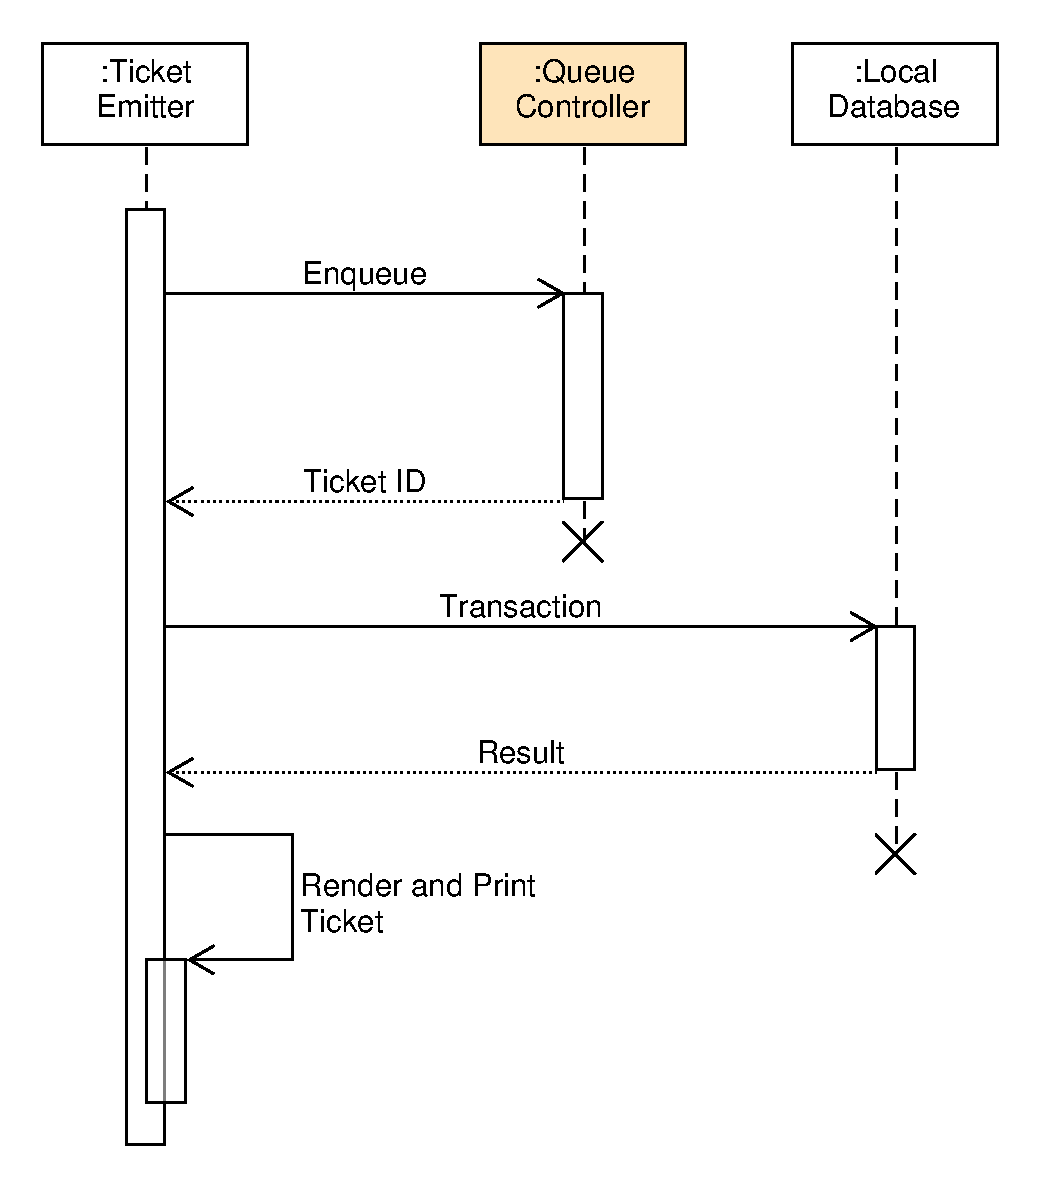
\includegraphics[width=\textwidth]{Images/UML_paper_ticket_sequence.pdf}
    \caption{\label{fig:UML_paper_ticket_sequence}Sequence diagram for store map loading}
\end{figure}
\begin{figure}[H]
    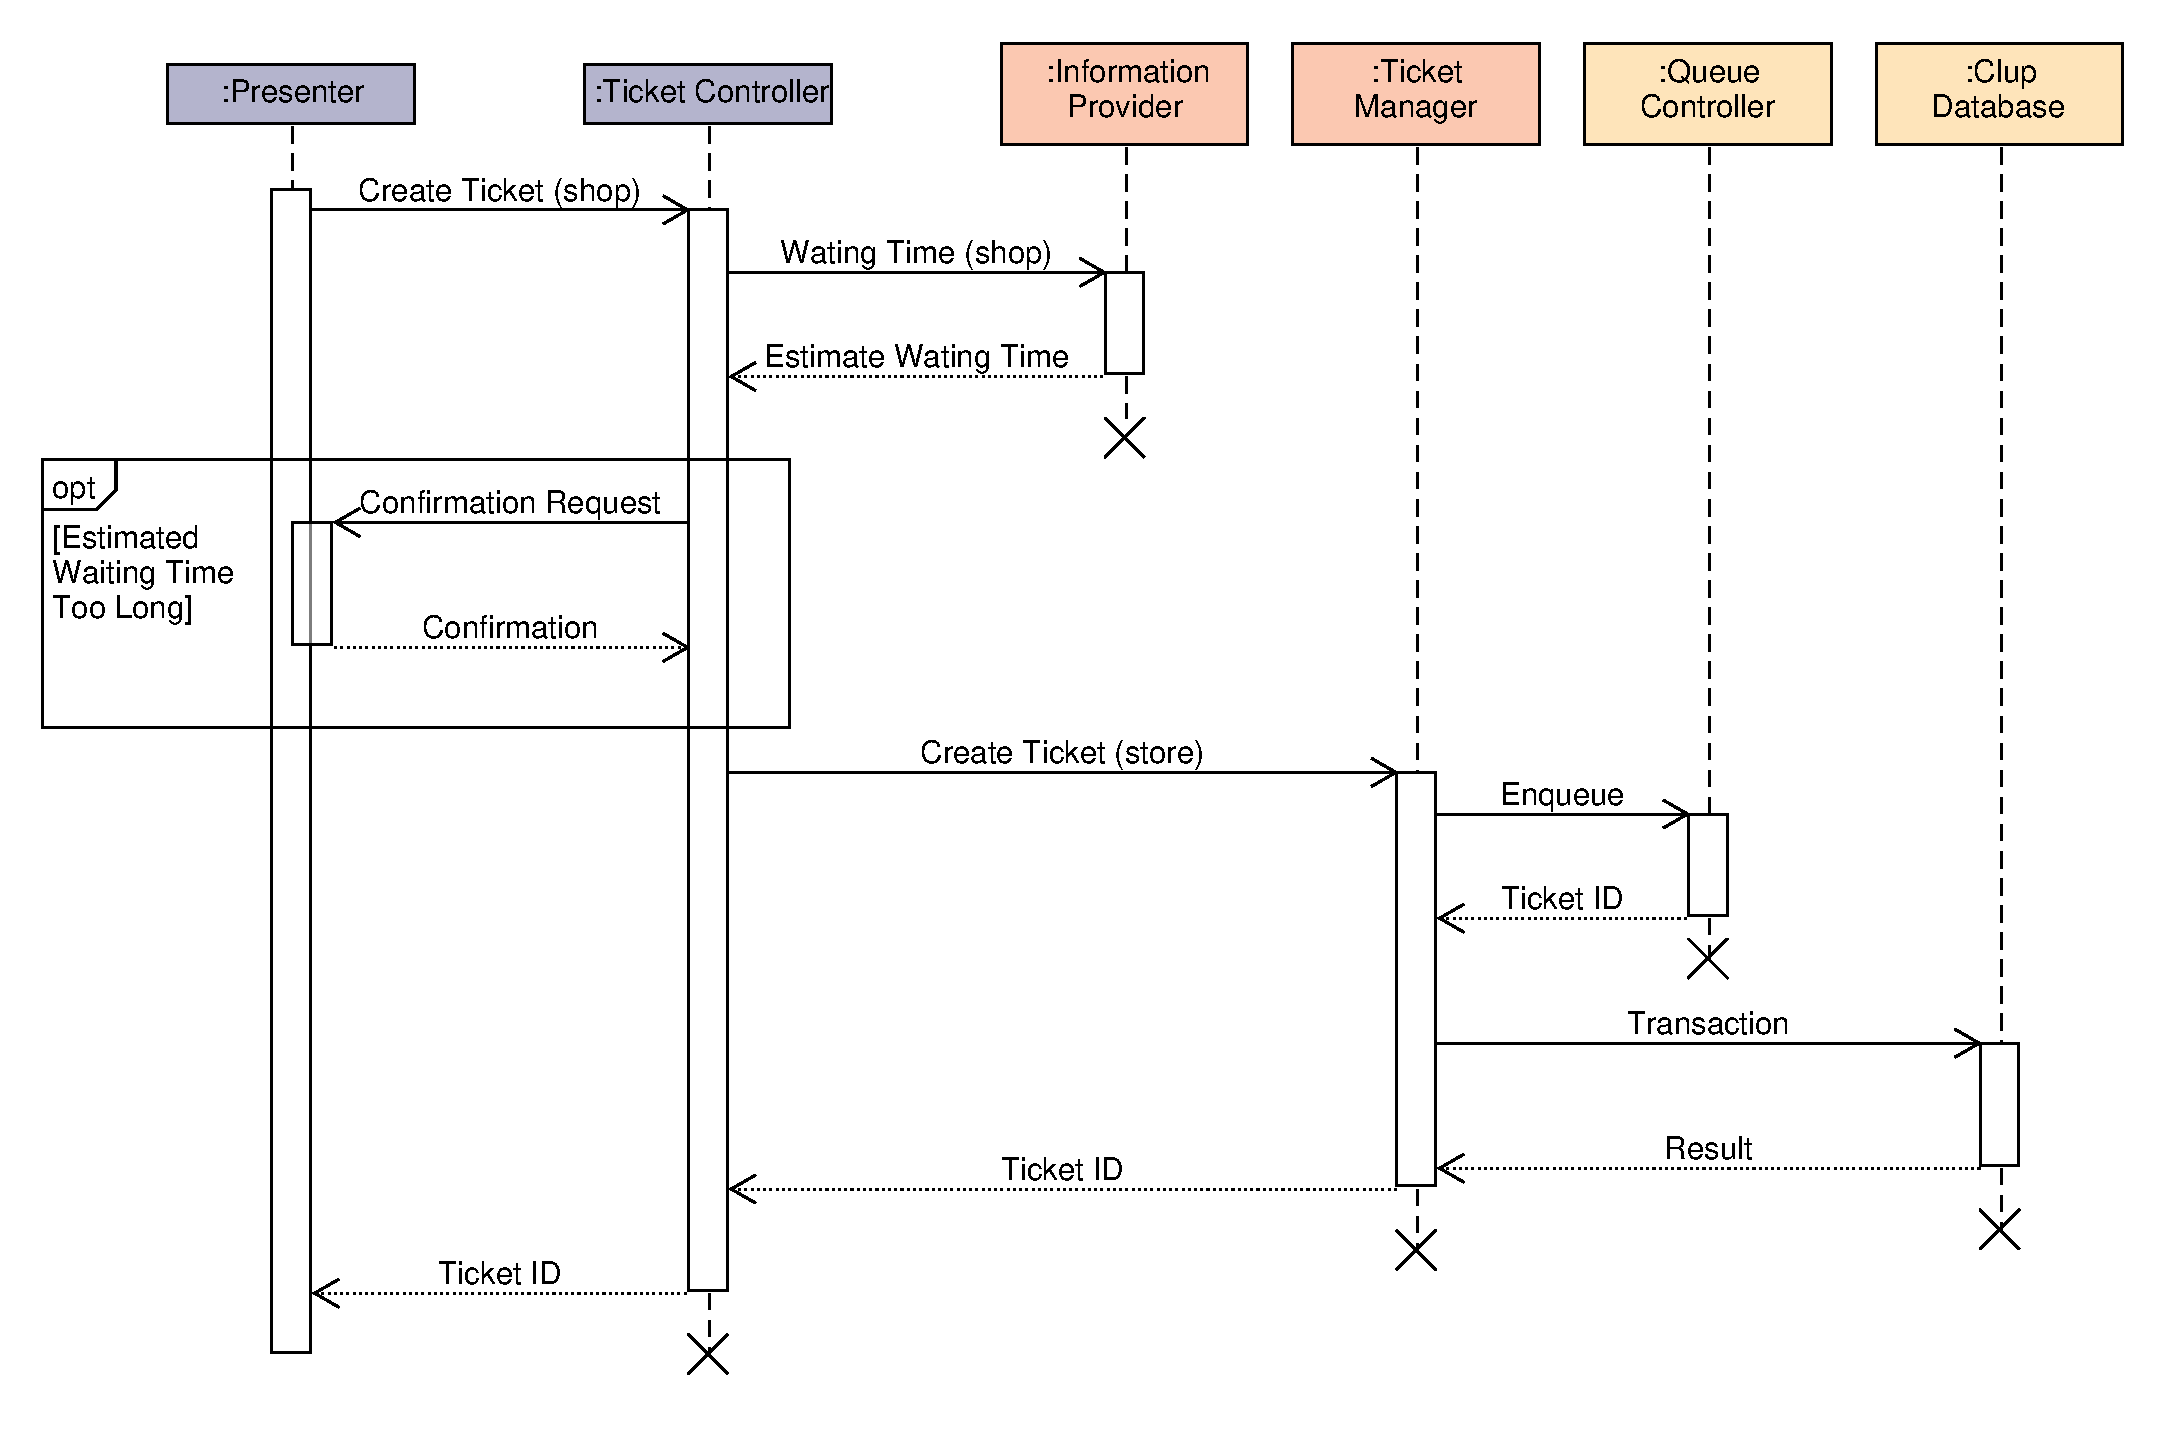
\includegraphics[width=\textwidth]{Images/UML_virtual_ticket_sequence.pdf}
    \caption{\label{fig:UML_virtual_ticket_sequence}Sequence diagram for store map loading}
\end{figure}
\subsection{Component Interfaces}

\subsection{Style Architecture}

% TODO: add section about relevant interfaces and algorithms is pseudocode